\documentclass[11pt]{report}
\usepackage{graphicx}
\usepackage{geometry}
\usepackage{titling}
\usepackage{fancyhdr}
\usepackage[latin1]{inputenc}
\usepackage{enumerate}
\usepackage{float}
\usepackage{latexsym}
\usepackage{amssymb}
\usepackage{amsthm}
\usepackage{amsfonts}
\usepackage{amsmath}
\usepackage[usenames,dvipsnames,svgnames,table]{xcolor}
\usepackage{listings}
\usepackage[hidelinks]{hyperref}
\usepackage[labelfont=bf]{caption}
\usepackage{longtable}
\usepackage{tablefootnote}
%\usepackage{tocbibind}
\parindent=0pt
\frenchspacing

\pagestyle{fancy}
\fancyhead[L]{\slshape\footnotesize December 3, 2014\\\textsc{02515 Health Care Technology}}
\fancyhead[R]{\slshape\footnotesize \textsc{Andreas Kjeldsen (s092638)}\\\textsc{Morten Eskesen (s133304)}}
\fancyfoot[C]{\thepage}

\newcommand{\tab}{\hspace*{2em}}
\newcommand{\HRule}{\rule{\linewidth}{0.5mm}}

\begin{document}

\begin{titlepage}
\begin{center}


\includegraphics[scale=2.0]{../GFX/dtu_logo.pdf}\\[1cm]

\textsc{\LARGE Technical University of Denmark}\\[1.5cm]

\textsc{\Large 02515 Health Care Technology}\\[0.5cm]


% Title
\HRule \\[0.4cm]
{\huge \bfseries Workout Memory Game}\\[0.1cm]
\HRule \\[1.5cm]

% Author and supervisor
\large
\emph{Authors:}
\\[10pt]
Andreas Hallberg \textsc{Kjeldsen}\\
\emph{s092638@student.dtu.dk}
\\[10pt]
Morten Chabert \textsc{Eskesen}\\
\emph{s133304@student.dtu.dk}

\vfill

% Bottom of the page
{\large December 3, 2014}

\end{center}
\end{titlepage}

\begin{abstract}
Overweight and obesity is an increasing problem in Denmark. Being physically active can prevent obesity and in turn make a person more healthy. We have created a game that requires the player to be active, by performing a sequence of exercises. The exercises must be performed in the right order and within a certain timeframe. The game has been build using Unity 3D and the Microsoft Kinect Sensor. The Kinect is used to track the player and to confirm the exercises are performed satisfyingly. We have tested our game on two group of kids in the age between 12 and 15. The tests showed an average increase in heart rate of 52.9\%.
\end{abstract}

\tableofcontents
\begingroup
\listoffigures
\let\clearpage\relax
\listoftables
\endgroup

\chapter{Introduction}
\section{Formalities}
This report is a result of a project done in the course \emph{Health Care Technology} taken at DTU. The project has been a collaboration between us both, Andreas and Morten, where we each have been equally responsible for all parts of the project. Andreas' mother works at an elementary school and by virtue of that we were able to test the game on kids from elementary school.

\section{Objectives}
The objective and product of the course Health Care Technology is to create a health-promoting interactive game by using Unity and Kinect technology. The game should solve a health care problem in Denmark. The course puts a lot of focus on health care challenges in today's Denmark and how the challenges can be solved by modern technology. In the future we will rely more and more on modern technology for health care problem as one of the problems in health care is the increasing need for treatment of the aging population. Another problem is the number of obese people in Denmark which has increased considerably in the last decade \cite{Sundhedsstyrelsen}.\\
This project aims to aid the solving of the increasing obesity problem in Denmark by creating a game that will increase the physical activity of people of age 13 and up, such that obesity can be prevented and obese people can become more healthy.

\section{Overweight \& obesity}
Overweight and obesity are defined as abnormal or excessive fat accumulation that presents a risk to health \cite{who-obesity}. An international measure known as Body Mass Index, henceforth \emph{BMI}, is commonly used to classify people as underweight, overweight and obese. BMI values are age-independent and the same for both sexes \cite{who-bmi}. BMI is calculated by the following:

$$\text{BMI}=\frac{\text{Weight (kg)}}{\text{Height}^2 \text{(m)}}$$
When calculating this you can use it to see if you are classified as underweight, normal, overweight or obese by the BMI scale. The BMI classifications and their corresponding values are defined as follows \cite{who-bmi}:
\begin{table}[H]
\centering
\caption{BMI classification}
\begin{tabular}{| c | c | c | c}
\hline
\textbf{Classification} & \textbf{BMI}\\ \hline
Underweight & Below 18.5 \\ \hline
Normal range & 18.5 - 24.99 \\ \hline
Overweight & Over 25\\ \hline
Obese & Over 30 \\ \hline
\end{tabular}
\end{table}
Overweight and obesity are major risk factors for a number of chronic diseases. These diseases include diabetes, cardiovascular diseases and cancer. In Denmark the total expenses linked with obesity and the treatment thereof on hospital was calculated as being 1.1 billion kroner in 2004 \cite{consequences-obese}.

\section{Memory}
There exists various ways to improving ones memory. One of the techniques is to exercise regularly. Many studies have shown that the parts of the brain that control memory and thinking have greater volume in people who exercise versus people who do not exercise \cite{harvard-health}. A study from University of California, Los Angeles showed that doing brain training games can significantly improve memory and language skills - especially in older people. The brain training programs can also delay dementia in later life \cite{dailymail}. Although the study used many different brain training games with different purposes, like reasoning, short- and long-term memory etc., we have decided to combine a brain training game with exercise. This has resulted in a game that combines a memory game with exercise.

\chapter{Game details}
\section{Game description}
The Workout Memory Game, as the name suggests, is a game where both memory and physical exercises are key components. The game consists of rounds, where in each round you have to perform certain exercises. The exercises are Squat and Jump. Round 1 consists of 1 exercise, Round 2 consists of 2 exercises - the previous one and a new exercise chosen at random and the game continues like this until game over.

\section{Requirements specification}
The focus of the game is to get people to exercise, hence it's vital to incorporate a requirement of movement. Though it might seem redundant, it is also important to make requirements on the visualization of the game, the difficulty of the game and the usability of the game.

\subsection{Game setup}
The game should be easy to setup. Hence there should be no additional software installations required to get the program working. There might be a small setup required for the actual room the game is to be played in. As this is a game that requires physical activity, the player should be able to move around, jump up and don and squat without hitting any obstacles. To enhance the gaming experience, the lights in the room should be turned on.

\subsection{Game start}
The player must be able to start the game just by interacting with the Kinect. When a game is finished, the player should be able to restart the game without having to first close down the game and then run it again.

\subsection{Player recognition}
The game must be able to recognize players\footnote{ To recognize a player, means identify that a player is in front of the Kinect. It does not mean identifying a specific person.}. The game must support one player, though two player mode would be nice to have. The game should support players of various height, width and depth, thus the game should be able to calibrate when a new player is recognized. The game should be able to detect if a player is missing and pause the game accordingly, though this should only be in effect between rounds to prevent cheating.

\subsection{Game progression}
While playing the game, the user should be able to determine if they're progressing or not. The game should consist of rounds, which the player can use to determine if they're progressing or not. The player should also be rewarded when progressing in the game. The reward should be points which in turn should increase the players score.

\subsection{Exercises}
The exercises the player has to perform should be picked at random. Picking the exercises at random forces the player to be paying attention and to exercise their memory. Each round a new exercise must be added to the sequence of exercises to perform. The order of the exercises must not be changed within a single game. The exercises are shown sequentially. The position on the screen where the exercise will be shown should be chosen at random the first time, in the following rounds the exercise should be shown at the same position.

\subsection{Gesture recognition}
The basis for the game, is that the player should perform a specific set of exercises. The game must be able to recognize these exercises. The game should also be able to recognize exercises that are being performed in a consecutive manner. The recognition should be flexible, in such a way that false positives for gestures are very rare and preferably not happening at all.

\subsection{Timing}
Each exercise should be performed within a set amount of time. When an exercise is performed correctly, the timing should be reset and allow the same amount of time for the next exercise. The amount of time should allow for the player to remember which exercise to perform and for the player to actually perform it. The amount of time should not allow for the player to write down the exercises, look up which to perform or become too relaxed.

\subsection{Scoring}
When the player is rewarded points for performing the right exercise, the amount of points being rewarded along with the exercise the user performed, should be shown on the screen. Showing the rewarded points and the exercise is a way for the game to provide feedback for the player. The feedback informs the player that the exercise was recognized and that they should progress onto the next exercise. The feedback should be shown on the screen where the exercise perform was shown. The amount of points gained should depend on how far the player has progressed in the game and how quickly they perform the exercise.

\subsection{Game over}
The game should end if an exercise is not performed within the allowed time or if the wrong exercise is performed. The player must be informed that the game is over. A summary of the game should be displayed to the player.

\subsection{Summary}
Below is a summary of the requirements specification modeled as a table. Each requirement states two scenarios, the \emph{need to have} and the \emph{nice to have}. As a minimum the game should support the need to haves, but we aim for the game to support most, if not all, of the nice to haves. 


\begin{center}
\begin{longtable}{| p{3cm} | p{4.75cm} | p{6cm} | }
\caption[Requirement specification summary]{Requirement specification, describing the minimum requirements (Need) and the desired requirements (Nice).}\\

\hline
\multicolumn{1}{|c|}{\textbf{Requirement}} & \multicolumn{1}{c|}{\textbf{Need}} & \multicolumn{1}{c|}{\textbf{Nice}} \\
\endfirsthead

\multicolumn{3}{c}%
{{\bfseries \tablename\ \thetable{} -- continued from previous page}} \\
\hline \multicolumn{1}{|c|}{\textbf{Requirement}} &
\multicolumn{1}{c|}{\textbf{Need}} &
\multicolumn{1}{c|}{\textbf{Nice}} \\
\endhead

\multicolumn{3}{r}{\textit{Continued on next page}} \\
\endfoot

\endlastfoot


\hline
Room setup & A well lit room with no objects within the viewport of the Kinect & A room with some lights turned on, doesn't matter if there are objects within the viewport of the Kinect \\ \hline
Game start & The player must able to start the game by interacting with the Kinect & The player must be able to both start and restart the game by interacting with the Kinect \\ \hline
Amount of players & One player is supported & Two players are supported \\ \hline
Player recognition & The game should be able to recognize the player, calibration poses might be required & The game should be able to recognize the player, calibration is done automatically \\ \hline
Player missing & The game should be able to detect if a player is missing and pause the game accordingly & The game should be able to detect if a player is missing and pause the game accordingly, but only between rounds, to prevent cheating \\ \hline
Game progression & The game consists of rounds which the player can progress though & The game consists of rounds which the player can progress through, additionally points are also rewarded \\ \hline
Exercises & New exercise each round while keeping the order of previous exercises, the exercises are all shown in the middle of the screen & New exercise each round while keeping the order of previous exercises, the exercises are shown at random positions \\ \hline
Gesture recognition & The gestures are recognized, false positives are rare & The gestures are recognized, false positives are very rare if not happening at all \\ \hline
Timing & Timing of exercise, player has plenty of time between exercises & Timing of exercises, player has little time between exercises and must remain active and observant. \\ \hline
Scoring & Points are earned when performing the right exercise & Points are earned when performing the right exercise, amount of points are based on game progression \\ \hline
Feedback & The player gets visual feedback when an exercise has been performed & The player gets visual feedback when an exercise has been performed while also being notified about the amount of points earned \\ \hline
Game over & The game can end when the player fails to perform the right exercise within the allowed time & The game can end when the player fails to perform the right exercise within the allowed time, the obtained score is also shown on the screen \\ \hline
\end{longtable}
\end{center}

\clearpage

\section{Technology}
The game has been developed using Unity 3D and the Microsoft Kinect Sensor technology.

\subsection{Unity 3D}
Unity 3D, henceforth Unity, is a Game Engine that can be used for developing games in both 2D and 3D. Unity includes a physics engine. In the Unity Asset Store, an enormous amount of community created assets are available, some have to be bought, others are available for free. The assets range from complete games to single assets with very specific functionality. Using the assets from the Asset Store can speed up the development process and also makes it possible to create good looking and functional games without skills in both design and coding.

\subsection{Microsft Kinect Sensor}
The Microsoft Kinect Sensor technology is capable of tracking human movements, by tracking a specific set of joints of the humanoid skeleton, see \autoref{fig:kinectjoints}. Specific limbs can also be tracked by using two or more tracked joints and calculating the movement of the limbs based on the joints.

\begin{figure}[H]
\centering
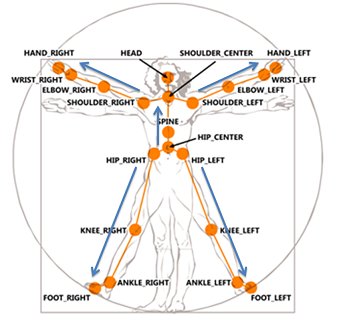
\includegraphics{../GFX/joints.png}
\caption[Joints trackable by the Microsoft Kinect Sensor technology]{The joints trackable by the Microsoft Kinect Sensor technology \cite{kinectjoints}\cite{kinectusertracking}.}
\label{fig:kinectjoints}
\end{figure}


\chapter{Implementation}
The game has been implemented using Unity3D Free v4.5.4 as the game engine, the Visual Studio IDE for coding in C\# and the Microsoft Kinect Sensor v1 for player tracking.  The game has been made in an incremental manner, using some of the principals of Scrum. Git and Github has been used for source control, feature discussion and issue tracking. 

\section{Scene}
The scene was kept simple. There's a skybox with a solid color used as the background for the game. GUIText objects are then used to display various texts. The game is to be kept simple and not overly fancy, therefore the texts are using a font with the look and feel of good old 8bit games. The font is readable close by and when it's scaled up. The font is called \emph{Press Start 2P} and is Open Font licensed (OFL) \cite{2pfont}. 

\section{Game management}
A set of classes were made to manage the game, these include a \emph{Brain} script, \emph{GameEventManager} script and \emph{GUIManager} script. These scripts make up the primary game functionality. The Brain script is in charge of starting a new game, creating new rounds, adding moves to perform while playing, keeping score and ending the game. The GUIManager is in charge of showing/hiding and updating the GUITexts used within the game. The GameEventManager is used for delegating messages about the state of the game (start game, end game, new round).

\section{Keyboard input}
The game can be played using the keyboard. This was implemented for the sake of testing the game management functionality without having to interact with the Kinect. Pressing the up arrow key indicates a Jump, pressing the down arrow key indicates a Squat and pressing the space bar indicates a new game is to be started.

\section{Kinect integration}
The Kinect had to be hooked up to the game. At first the KUInterface code that was handed out in the course was used to interact with the Kinect. It worked, but was missing some functionality that was required, hence another wrapper for interacting with the Kinect was found on the Unity Asset Store \cite{assetstorekinect}. The other wrapper included a KinectWrapper class that is in charge of communicating with the Kinect using PInvoke calls and a KinectManager class to be used with Unity. The KinectManager included a large amount of code for gesture recognition that was overly complicated, hence the code has been removed together with several options of the KinectManager that was of no use.

\section{Joint tracking}
The KinectManager provides functionality for obtaining the current positions of the joints in \emph{Viewport Space}. To verify that the joints are tracked, GameObjects were setup to follow the joints. GameObjects use \emph{World Space}, hence the joint position had to be changed into World Space. The calculations required for transforming the positions were included with the KinectManager \cite{assetstorekinect}. A class for tracking all the joints and overlaying them with GameObjects were made, further a helper class for obtaining, getting and setting the joint positions were made, this also allowed for logging of the joint positions to a log file.

\section{Gesture recognition}
The joints are tracked in Viewport Space, which is a 2 dimensional space and goes from -1.0 to 1.0 in both the $x$ and the $y$ direction. There are no certainties that the joints are always at the same height when the player is idle, i.e. the \emph{HipCenter} joint is not always located at $y = 0.0$. The joint position logging was then used to find a base interval in which it could be assumed that the HipCenter joint was located when the player is idle. Same procedure for the other joints used in the jump gesture (KneeLeft, KneeRight), the squat gesture (KneeLeft, KneeRight, HipLeft, HipRight) and the clap gesture (HandLeft, HandRight). To actually be a gesture, the player had to perform a specific action. When jumping, the player have to raise their knees a certain amount, when squatting the player has to lower their knees and hips a certain amount and when clapping the player has to move their hands together. The amount the joints had to move was also found using the joint positions log. By performing the exercises while logging the joint positions, the goal intervals in which it could be assumed the player would have reached the required pose was found. Using the base intervals and the goal intervals, the amount required to move the joints were found. Detecting a gesture was then just the matter of tracking the joints required in the gesture over time, noting if the joints moved by the required amount. Restrictions are in place, stating that the player has to be within the base intervals for the joints before a gesture is tracked. This is e.g. to prevent two simultaneous squats to be perceived as a jump.

\begin{figure}[H]
\centering
	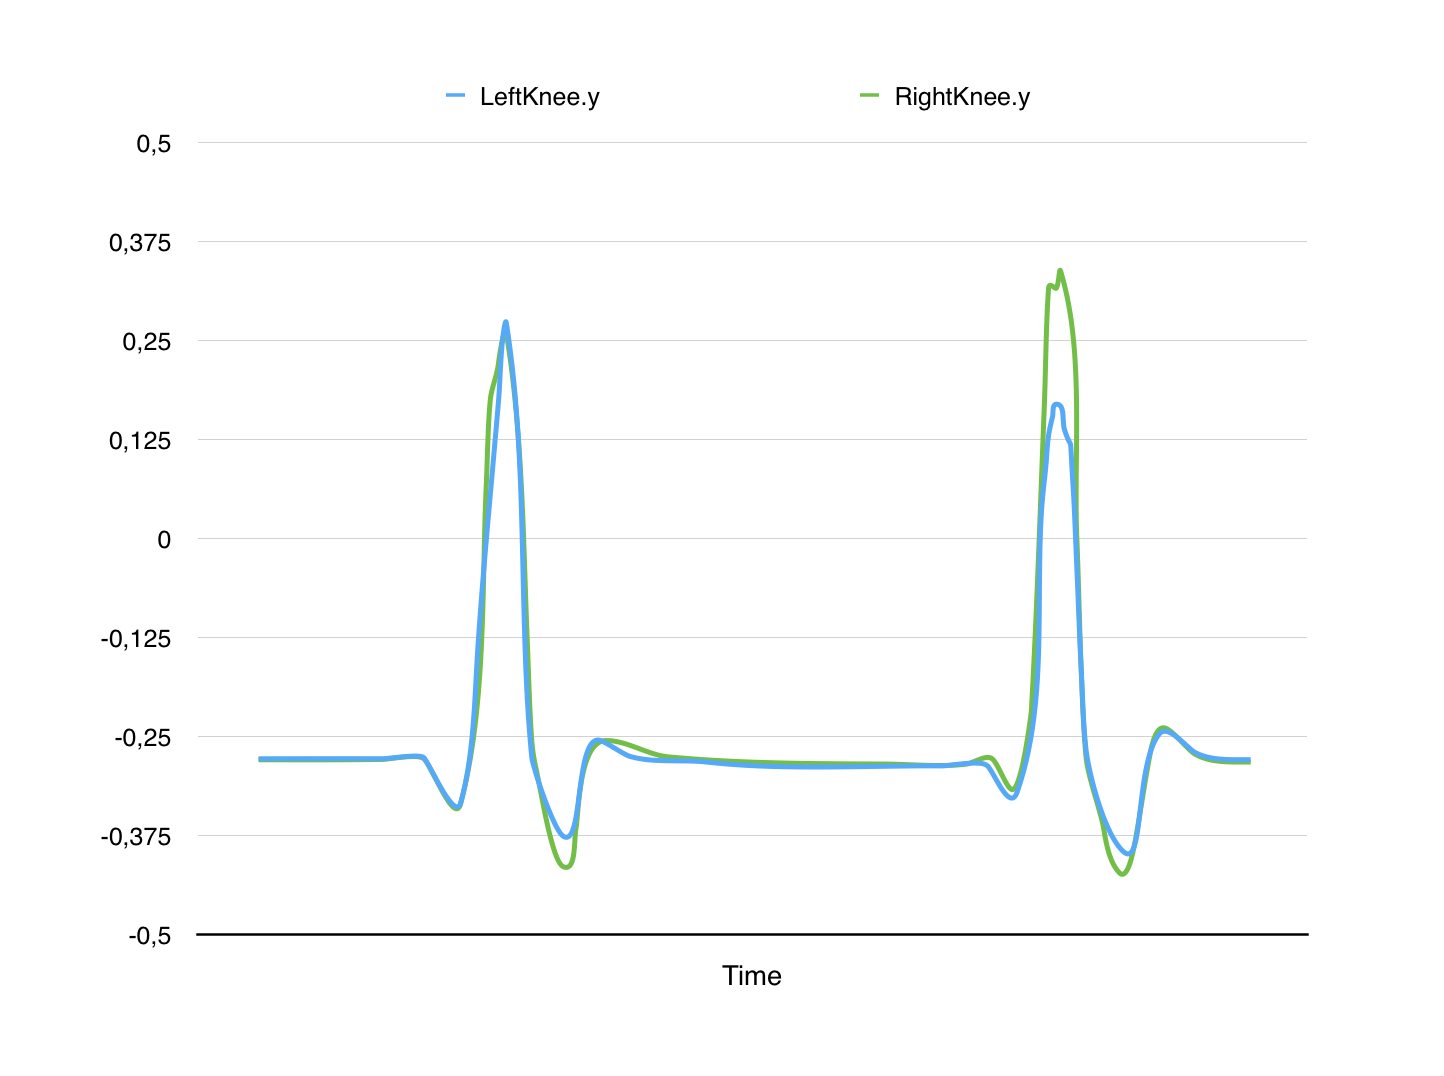
\includegraphics[scale=0.6]{../GFX/Trackinggraph.png}
\caption[Graph depicting joint tracking of KneeLeft and KneeRight]{Graph showing the positions of the joints KneeLeft and KneeRight during a session where the player jumped.}
\end{figure}

\section{Visual improvements}
The primary visual used in the game is the feed from the RGB camera of the Kinect. The texts used was clear and readable when just testing the Game Management, as the background was a solid color and the texts was another solid color with great contrast. When using the feed from the RGB camera as the background of the game, there are no limits to the colors, shapes and lightning. Therefore a border was added to the text. In Unity 3D Free v4.5.4 the GUIText component does not have a border feature. To fix this, a script was made mimics a border around the text, by drawing the text multiple times behind the actual GUIText. While developing the game, a preview screen is visible that shows what the game will look like. Everything seems fine in the preview, but when the game is launched and played in full screen mode, the texts weren't scaling, hence they were quite hard to read from a distance. Another script was created that scales the texts. A third script was created, which makes the texts fade out after a certain amount of time.

\chapter{Test}
This chapter will outline our test specification and the test results from testing on children from an elementary school. Lastly it will discuss the test results in regards to the test specification.

\section{Test specification}
In this section we have modeled our test specification as a table. Each test states two scenarios, the \emph{need} to have and the \emph{nice} to have. The needs to have describe the minimum acceptance criteria and the nice to have describe the desired acceptance criteria.

\begin{center}
\begin{longtable}{| p{1cm} | p{3.2cm} | p{3.75cm} | p{3.75cm} |}
\caption[Test specification]{Test specifcation, describing the minimum acceptance criteria (Need) and the desired acceptance criteria (Nice).}\\

\hline
\multicolumn{1}{|c|}{\textbf{ID}} & \multicolumn{1}{|c|}{\textbf{Test}} & \multicolumn{1}{c|}{\textbf{Need}} & \multicolumn{1}{c|}{\textbf{Nice}} \\
\endfirsthead

\multicolumn{4}{c}%
{{\bfseries \tablename\ \thetable{} -- continued from previous page}} \\
\hline
\multicolumn{1}{|c|}{\textbf{ID}} & \multicolumn{1}{|c|}{\textbf{Test}} & \multicolumn{1}{c|}{\textbf{Need}} & \multicolumn{1}{c|}{\textbf{Nice}} \\
\endhead

\multicolumn{4}{r}{\textit{Continued on next page}} \\
\endfoot

\endlastfoot

\hline
T1 & Start \& setup time & 1 min & 30 seconds \\ \hline
T2 & User interface & User is instructed and can play & User can play without instructions \\ \hline
T3 & Game progression & Game progression is reported & Difficulty of game is adapted to how far the player has progressed in the game\\ \hline
T4 & Jump recognition & A jump is recognized & Height of a jump is recognized \\ \hline
T5 & Squat recognition & A squat is recognized & A deep squat is recognized \\ \hline
T6 & Clap recognition & A single clap is recognized & A double clap is recognized \\ \hline
T7 & Calibration & User has to stand in specific pose to calibrate & Calibration is done automatically \\ \hline
T8 & Player's heart rate & 20\% increase in heart rate of player on average & 40\% increase in heart rate of player on average \\ \hline
T9 & Player's memory & The player at least stays at the same round & The player progresses at least 1 round, as long as their physique allows it \\ \hline
T10 & Missing player & If no player is detected, the game should pause & If no player is detected, the game should pause and notify about the player missing \\ \hline

\end{longtable}
\end{center}

\section{Test results}
Besides testing on ourselves, our friends and family, we also wanted to take the game out in the world and apply it in an environment where it could possibly have a positive effect. Our game was tested on kids in age range 12-15 at an elementary school in Helsing\o r. The game was tested in a classroom, hence we could test if furniture in the background would interfere. We found that the player had to stand at least 12 meters away and be right beside some furniture, before it would have an effect on the Kinect registering the joints properly. One of the measurable features of a training game is the heart rate of the player. When testing we noted the heart rate of the player before and after playing the game. What follows is a table of the test results obtaining from the elementary school.\\
\\
Players occurring with the same name are not different players but the same player's second try. The first number in the heart rate column is the heart rate before and the second number is the heart rate after - i.e. 76 $\rightarrow$ 114 means a heart rate of 76 before and 114 after playing. The percentage describes how much the heart rate increased in percentage. FR is Failure Reason where the following codes apply:
\begin{itemize}
\item[1] Wrong exercise done by the player
\item[2] Time ran out, i.e. no exercise was done in time
\item[3] Registration error
\item[4] Computer crashed
\end{itemize}

\begin{table}[H]
\centering
\caption[Test results]{Results after testing 14 kids with an average age of 13.9. The results show an average increase in heart rate of 52.9 \%.}
\begin{tabular}{ | c | c | c | c | c | c | c | c | c | c |}
\hline
\textbf{Name} & \textbf{Age} & \textbf{Gender} & \textbf{Heart rate} & \textbf{Diff.} & \textbf{\%} & \textbf{Round} & \textbf{Score} & \textbf{FR}\\ \hline
Amine & 15 & F & 76 $\rightarrow$ 114 & 38 & 50.0 & 5 & 2264 & 1\\ \hline 
Anders & 15 & M & 64 $\rightarrow$ 93 &  29 & 45.3 & 3 & 253 & 1\\ \hline 
Anders & 15 & M & 67 $\rightarrow$ 102  & 35 & 52.2  & 4 & 1057 & 1\\ \hline 
%Andreas & 24 & M & 72 $\rightarrow$ 163 &  & y & 17 & 86505 & \\ \hline 
Ditte & 14 & F & 69 $\rightarrow$ 117 & 48  & 70.0 & 9 & 10045 & 4\\ \hline 
Ditte & 14 & F & 74 $\rightarrow$ 141 & 67 & 90.5 & 12 & 27497 & 1\\ \hline 
Frederik & 15 & M & 73 $\rightarrow$ 94 & 21 & 28.8 & 3 & 342 & 2\\ \hline 
Freja & 13 & F & 72 $\rightarrow$ 80 &  8 & 11.1 & 2 & 58 & 1\\ \hline 
Freja & 13 & F & 77 $\rightarrow$ 96 &  19 & 24.7 & 3 & 143 & 3\\ \hline 
Imon & 15 & M & 78 $\rightarrow$ 100 & 22 & 28.2 & 5 & 1971 & 1\\ \hline 
Isabella & 15 & F & 73 $\rightarrow$ 120 & 47 & 64.4 & 7 & 6132 & 1\\ \hline 
Jasper & 15 & M & 71 $\rightarrow$ 87  & 16 & 22.5 & 3 & 652 & 1\\ \hline 
Jasper & 15 & M & 73 $\rightarrow$ 123 & 50 & 68.5 & 7 & 6129 & 1\\ \hline 
L\ae rke & 12 & F & 79 $\rightarrow$ 106 & 27 & 34.2 & 4 & 1077 & 3\\ \hline 
L\ae rke & 12 & F & 73 $\rightarrow$ 121 & 48 & 65.8 & 11 & 18528 & 1\\ \hline 
Marcus & 12 & M & 76 $\rightarrow$ 114 & 41 & 54.0 & 4 & 3308 & 1\\ \hline 
Marcus & 12 & M & 73 $\rightarrow$ 132 & 59 & 80.8 & 13 & 36939 & 1\\ \hline 
Nicklas & 15 & M & 64 $\rightarrow$ 104 & 40 & 62.5 & 5 & 1983 & 1\\ \hline 
Nicklas & 15 & M & 73 $\rightarrow$ 114 & 41 & 56.2 & 8 & 6931 & 1\\ \hline 
Philip & 13 & M & 73 $\rightarrow$ 127 & 54 & 74.0 & 9 & 10116 & 1\\ \hline 
Philip & 13 & M & 78 $\rightarrow$ 141 & 63 & 80.8 &12 & 22991& 1\\ \hline 
Siw & 15 & F & 74 $\rightarrow$ 123 & 49 & 66.2 & 5 & 1411 & 2\\ \hline 
Siw & 15 & F & 72 $\rightarrow$ 129 & 57 & 79.2 & 12 & 19345 & 1\\ \hline 
Zenah & 13 & F & 74 $\rightarrow$ 91 & 17 & 23.0 & 4 & 1304 & 1\\ \hline 
Zenah & 13 & F & 83 $\rightarrow$ 112 & 29 & 34.9 & 8 & 9775 & 1\\ \hline
Average & 13.9 & \multicolumn{2}{r}{} & & 52.9 & 6.9 & 7927.1 & \\ \hline
\end{tabular}
\end{table}

\begin{figure}[H]
	\centering
	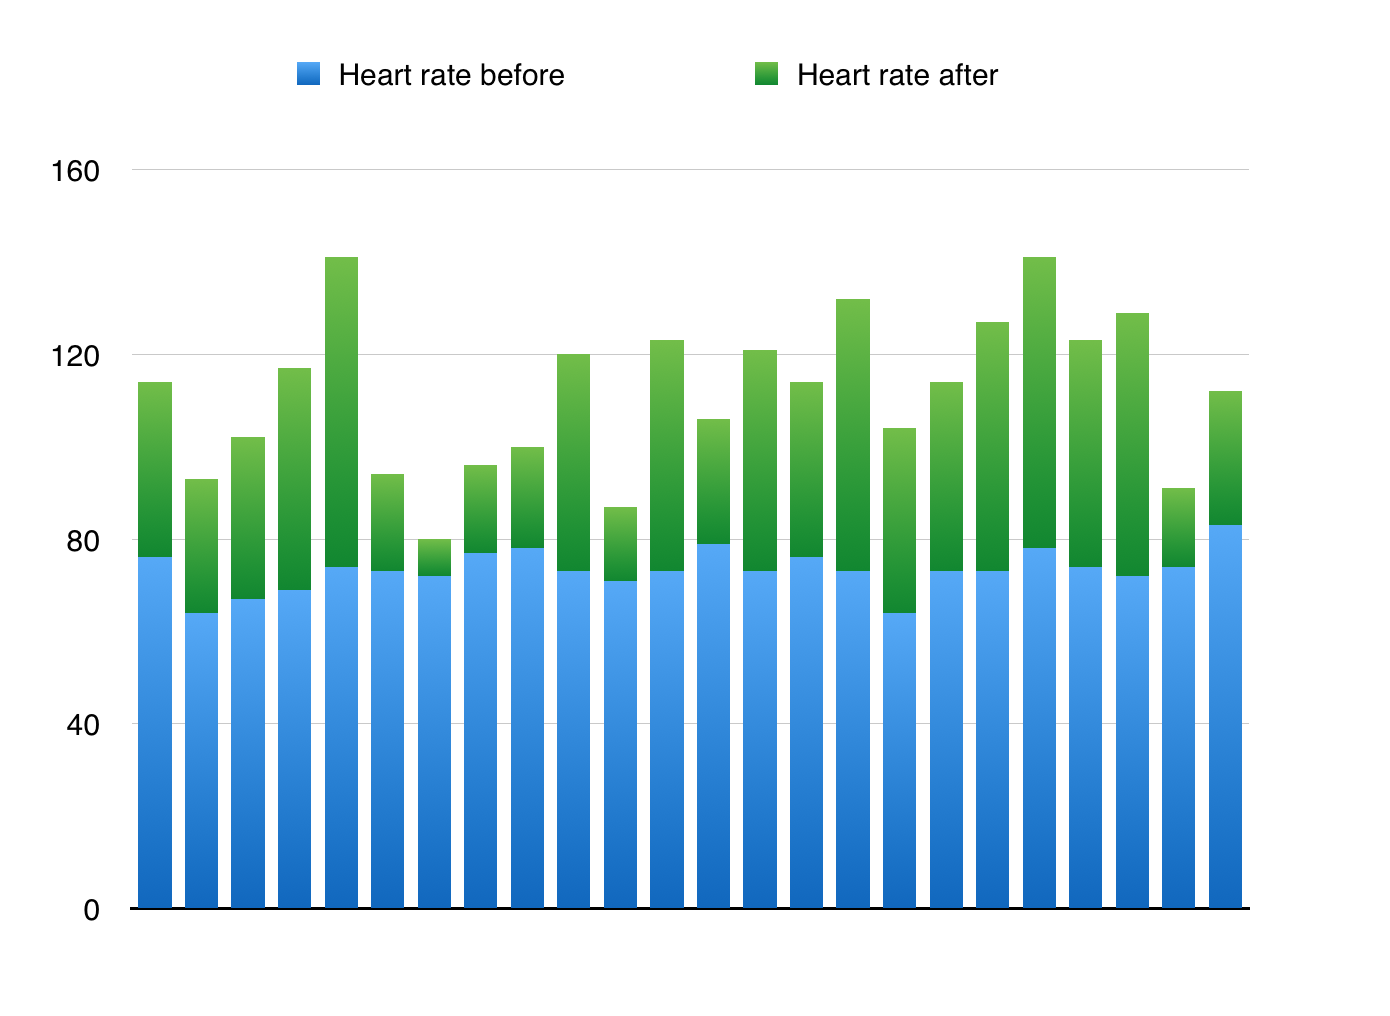
\includegraphics[scale=0.6]{../GFX/Resultsgraph.png}
	\caption{Graphical overview of the test results}
\end{figure}

\subsection{Feedback}
The children playing our game gave a lot of feedback to the game. As a spectator you could very clearly see that they were trying hard to remember the exercises especially in the higher rounds. What follows is a list of feedback given by the children.
\begin{itemize}
\item It is physically exhausting
\item You could clearly see when an exercise was done correctly by virtue of the green text on the screen with the points gained
\item It is hard to remember the order of exercises, especially when the exercises alternate very often
\item It is like using a Jump Rope (said by a girl who had many jumps)
\item At first it was difficult to tell how high to jump and how low to squat in order for the game to register the exercise properly
\item There is no sound, some background music would be nice
\end{itemize}

\begin{figure}[H]
\centering
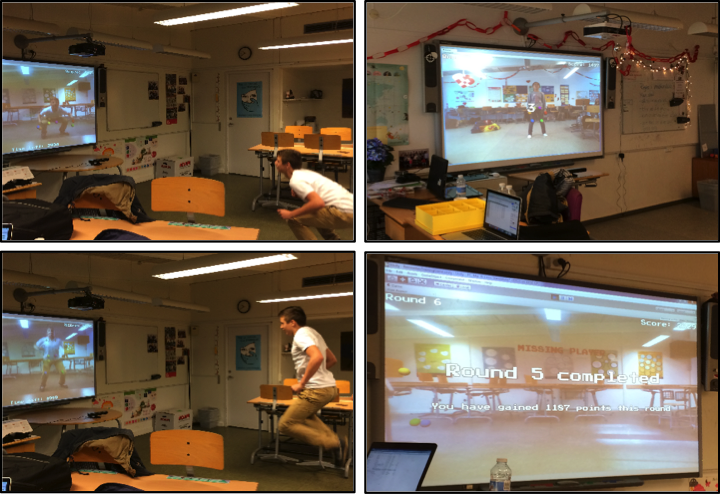
\includegraphics[scale=.59]{../GFX/UserTestingCollage.png}
\caption{Pictures from the test session}
\end{figure}

\section{Discussion}
Based on the test results, the following discussion will analyze to which extend the tests in the test specification have been passed.

\subsection*{T1: Start \& setup time}
The test session showed that the game was never more than 30 seconds to startup and be ready for playing. This means that we have achieved the \textbf{nice} criteria of this test case. However the only reason the startup took some time was because of the Kinect having to be started and therefore we would have liked a more smooth transition such as turning on a PlayStation so the screen is not all black when starting up.

\subsection*{T2: User interface}
During the test session the users were given a short introduction, explaining they had to jump if the game said jump and squat if the game said squat. Even without further introduction, it was clear that the users quickly understood how the gesture recognition feedback worked, how high to jump and how deep to squat. The game states the commands to perform but may lack further explanation of when and how to jump and squat. The test case only satisfies the \textbf{need} criteria.

\subsection*{T3: Game progression}
The requirements for the gestures are not becoming more strict the further the player has progressed. But the amount of exercises to remember is increased, so in a sense, the difficulty of the game is adapting to the performance of the player. Further it could be introduced that the previous exercises are either not shown again or the time they are shown is decreased. The test case only satisfies the \textbf{need} criteria.

\subsection*{T4: Jump recognition}
If the height of a jump had been recognized we could have logged the heights of all the jumps made by players. We could have used this to make an analysis of how high each player jumps and who had the record among the test subjects. As mentioned the requirements for jumping are not becoming more strict as the game is progressing. We would have liked to have done this in order to make the game more difficult as the game progressed such that the player had to jump higher and higher. The test case satisfies the \textbf{need} criteria.

\subsection*{T5: Squat recognition}
Requiring that the player was to do a deep squat was definitely possible code-wise, but during our test session, it showed that not all people are flexible enough to actually do a deep squat, thus the requirement for the squat was slacked a bit. With the requirement slacked, the player can still perform a deep squat and it will still be recognized. Encouragement towards performing the exercises to their full extent should be a part of the introduction to the game. The test case satisfies the \textbf{nice} criteria.

\subsection*{T6: Clap recognition}
The test showed that a single clap to start the game could be confusing. It is not uncommon for people to put their hands together, just as if they would clap. Requiring a double clap proved to be more appropriate, as it had to be a conscious action performed by the player. The test case satisfies the \textbf{nice} criteria.

\subsection*{T7: Calibration}
The test session showed that we did not have to restart the game between each player or position each player in a specific pose in order to calibrate. The calibration was done automatically. The test case satisfies the \textbf{nice} criteria.

\subsection*{T8: Player's heart rate}
The test session yielded a result that showed an average of 52.9\% increase in heart rate. This is a quite high increase in heart rate for a game. It has to be taken into account that the test subjects were quite excitable and very competitive with their friends and laughing while playing. Therefore we can not point out the game as the single factor for the increase in heart rate. However the test case satisfies the \textbf{nice} criteria, which was a 40\% increase in heart rate.

\subsection*{T9: Player's memory}
The test session showed that each player who tried the game more than once progressed at least 1 more round the second time than their first time. It means that the players are getting better and better at the game and thereby doing more exercises and increasing their heart rate and their ability to remember the exercises to perform. The test case satisfies the \textbf{nice} criteria. 

\subsection*{T10: Missing player}
The test session showed that each time a player was not able to be registered then the game notified that a missing player was missing and paused the game. This was however only done between rounds, i.e. before exercises for the round is being shown on the screen in order to prevent players from cheating by writing down the order of exercises. The test case satisfies the \textbf{nice} criteria.

\chapter{Conclusion \& Discussion}
This chapter will conclude and discuss the work done in this project. It will also discuss the possibilities for further development of the game.

\section{Conclusion}
In this project we have used Unity and Kinect technology to create a game that challenges both the memory and the fitness of the player. The game combines the two physical exercises Jump and Squat to create a Workout Memory Game. The game consists of rounds. Round 1 consists of 1 exercise, round 2 consists of the previous exercise and a new exercise and so on until the game is over. The exercises are chosen at random. The player has 5 seconds to perform each exercise and the game ends when a player runs out of time to do an exercise or doing the wrong exercise. The game has fulfilled all the desired requirements from the requirement specification excluding the desired requirement about two player mode. The test results showed an average of 52.9\% increase in heart rate, which is more than our initial desired acceptance criteria. The test results also showed that the players also progressed further in the game for each time they played the game.

\section{Further development}
The vision for the game is to extend it into a suite of small games to help the player exercise. The Workout Memory Game should just be one of the small games included in the suite. The other small games could then focus on something else like the arms, suppleness or reaction time. Introducing two player mode would also be a possibility, this way the player not only competes with themselves but also a friend (or foe). As a suite, the players would have a profile where they stats would be logged. The player should then be able to track their progress in the various small games. Based on the player progression, the games should become either harder or easier to allow for further improvement. Ideally the suite could be linked with various apps like Endomondo and gadgets like the Nike FuelBand to collect even more data, that would be used for player statistics and progression overviews. Visually the suite would also need an overhaul and have a proper interface for navigating the system and exercises. As the game is implemented now each exercise to perform in every round is shown for 2 seconds. In order to introduce more difficulty this could be changed such that only the exercise introduced in the current round was shown for 2 seconds and the others for 1 second. Other possibilities could be that the number of time exercises are shown decreases as the game is processing. The introduction of sounds and music could make the experience even better. Sounds when performing the right exercise as another way to provide feedback and some background music to set people in the right mood.


\begin{thebibliography}{99}
\bibitem{Sundhedsstyrelsen}
  Sundhedsstyrelsen,
  \emph{Overv\ae gt}
  \url{http://sundhedsstyrelsen.dk/da/sundhed/overvaegt}

\bibitem{who-obesity}
	World Health Organization,
	\emph{Obesity}
	\url{http://www.who.int/topics/obesity/en/}
	
\bibitem{who-bmi}
	World Health Organization,
	\emph{BMI classification}
	\url{http://apps.who.int/bmi/index.jsp?introPage=intro_3.html}

\bibitem{consequences-obese}
	Ministeriet for Sundhed og Forebyggelse,
	\emph{Samfunds\o konomiske konsekvenser af sv\ae r overv\ae gt}
	\url{http://www.sum.dk/Aktuelt/Nyheder/Forebyggelse/2007/Maj/Samfundsoekonomiske_konsekvenser.aspx}

\bibitem{harvard-health}
	Heidi Goodman, \emph{Regular exercise changes the brain to improve memory, thinking skills}
	\url{http://bit.ly/1ewiOfg}
	
\bibitem{dailymail}
	Victoria Woollaston, \emph{Proof that brain training games DO boost memory and language skills in older people}
	\url{http://dailym.ai/1yGGhag}

\bibitem{kinectjoints}
	Microsoft Kinect SDK, \emph{JointType Enumeration}, viewed October 2014.
	\url{http://msdn.microsoft.com/en-us/library/microsoft.kinect.jointtype.aspx}

\bibitem{kinectusertracking}
	Microsoft Kinect SDK, \emph{Tracking Users with Kinect Skeletal Tracking}, viewed October 2014.
	\url{http://msdn.microsoft.com/en-us/library/jj131025.aspx}

\bibitem{2pfont}
	Google Fonts, \emph{Press Start 2P}
	\url{https://www.google.com/fonts/specimen/Press+Start+2P}
	
\bibitem{assetstorekinect}
	RF Solutions, \emph{Kinect with MS-SDK}, v1.11, October 15, 2014
	\url{https://www.assetstore.unity3d.com/en/#!/content/7747}

\end{thebibliography}

\end{document}
